\section{Sprint 1}

\subsection{Sprint Planning}

Velocidade do Time: 15~pessoas·hora.

Objetivo da Sprint: Estruturar a base de fontes bibliográficas para o projeto, definindo critérios de seleção e selecionando as três fontes principais.

\begin{table}[htbp]
  \centering
  \caption{Sprint backlog e tarefas — Sprint 1}
  \label{tab:sprint1}
  \begin{tabular}{ccc}
    \toprule
    Tarefa & Descrição & Estimativa (pessoas·hora) \\
    \midrule
    US-01A & Buscar fontes em bases científicas & 6 \\
    US-01B & Filtrar fontes relevantes & 7 \\
    US-01C & Selecionar 3 principais fontes & 2 \\
    \bottomrule
  \end{tabular}
  \fonte{Elaboração própria.}
\end{table}

\vspace{0.5em}
\noindent\textbf{Capacidade utilizada:} 15 pessoas·hora (100\% da velocidade da equipe)

\subsection{Quadro Kanban}

Histórico da evolução do quadro Kanban no início e ao final de cada Sprint.

\begin{figure}[htbp]
  \centering
  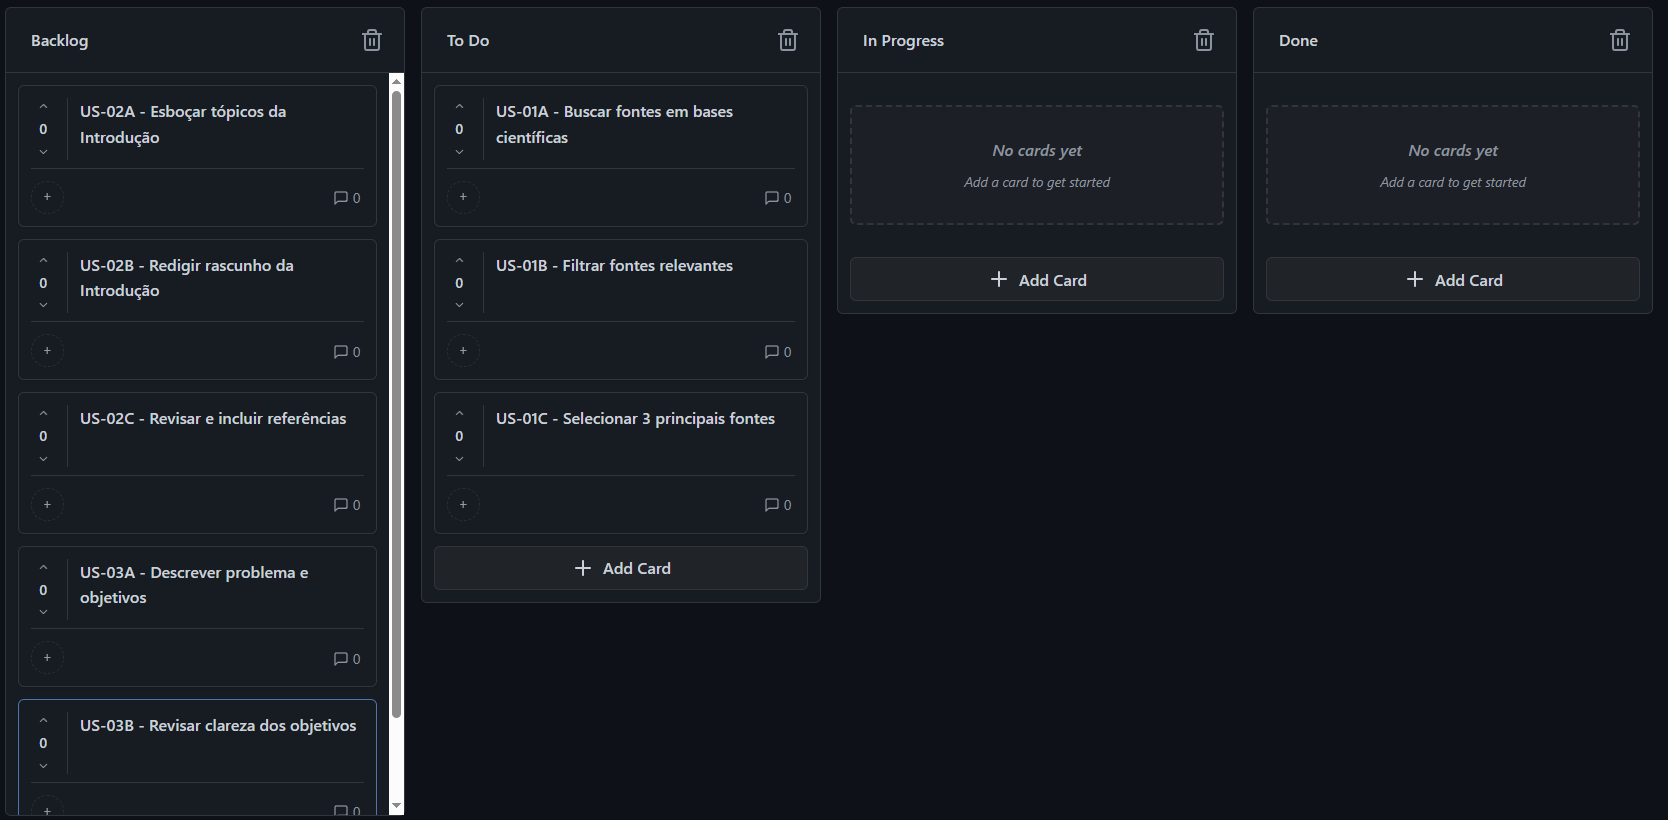
\includegraphics[width=0.8\linewidth]{pictures/kanban_sprint1_inicio.png}
  \caption{Visão geral do Quadro Kanban no início da Sprint 1}
\end{figure}

\begin{figure}[htbp]
  \centering
  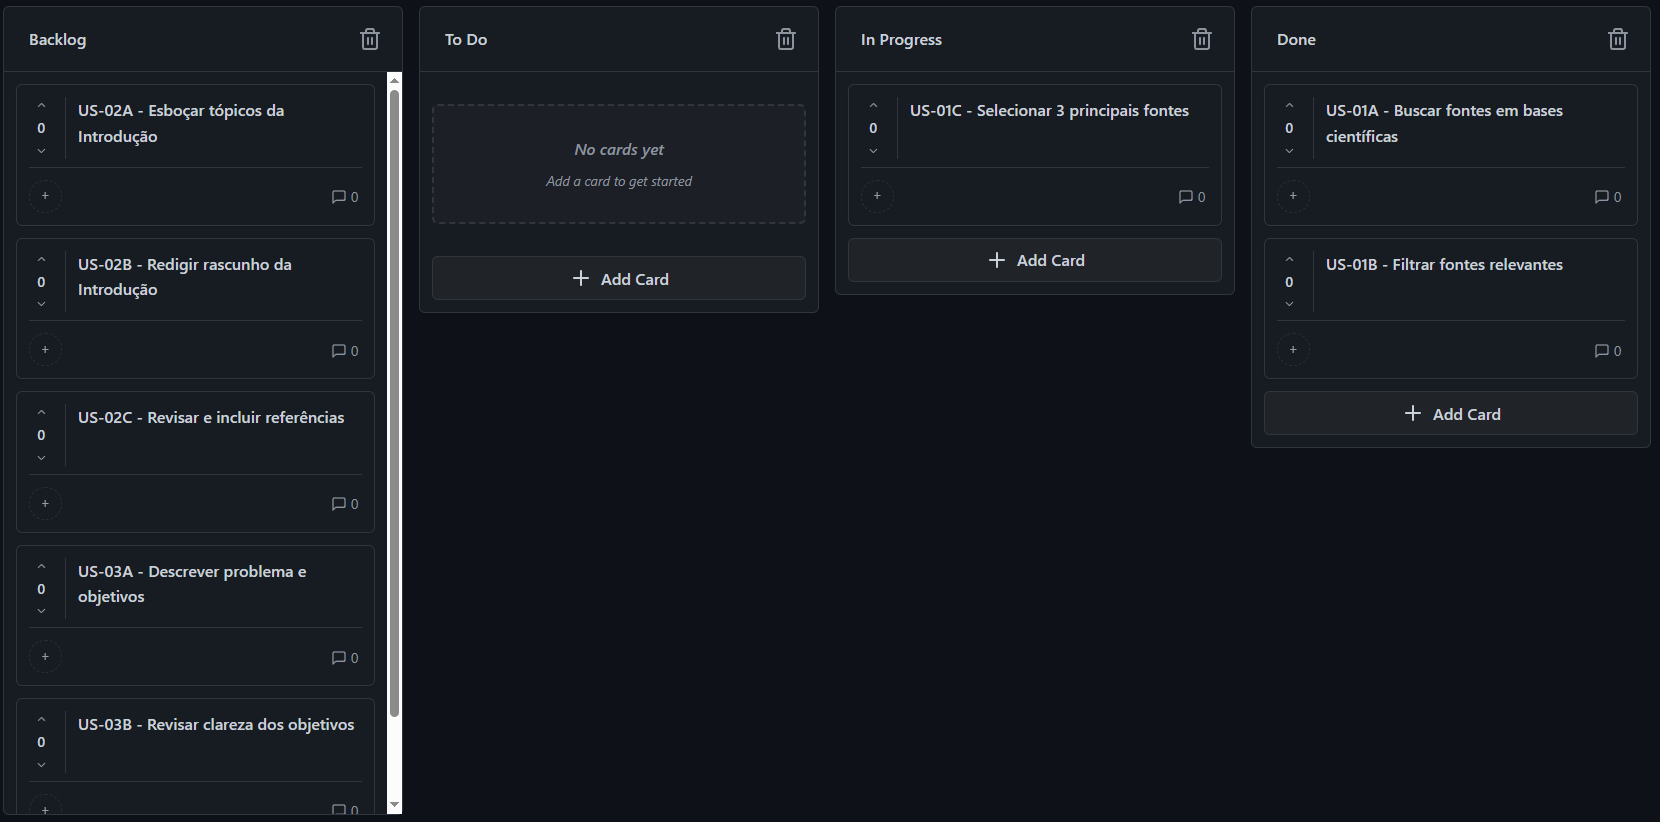
\includegraphics[width=0.8\linewidth]{pictures/kanban_sprint1_final.png}
  \caption{Visão geral do Quadro Kanban ao final da Sprint 1}
\end{figure}

\subsection{Reuniões de Acompanhamento}

Daily 1 (12/06/2025): Discutimos os critérios para filtragem de artigos e as ferramentas de busca mais eficazes.

Daily 2 (14/06/2025): Falta apenas a tarefa US-01C; Nota do futuro: a tarefa restante foi concluída em 17/06/2025, antes da retrospectiva.

\begin{figure}[htbp]
  \centering
  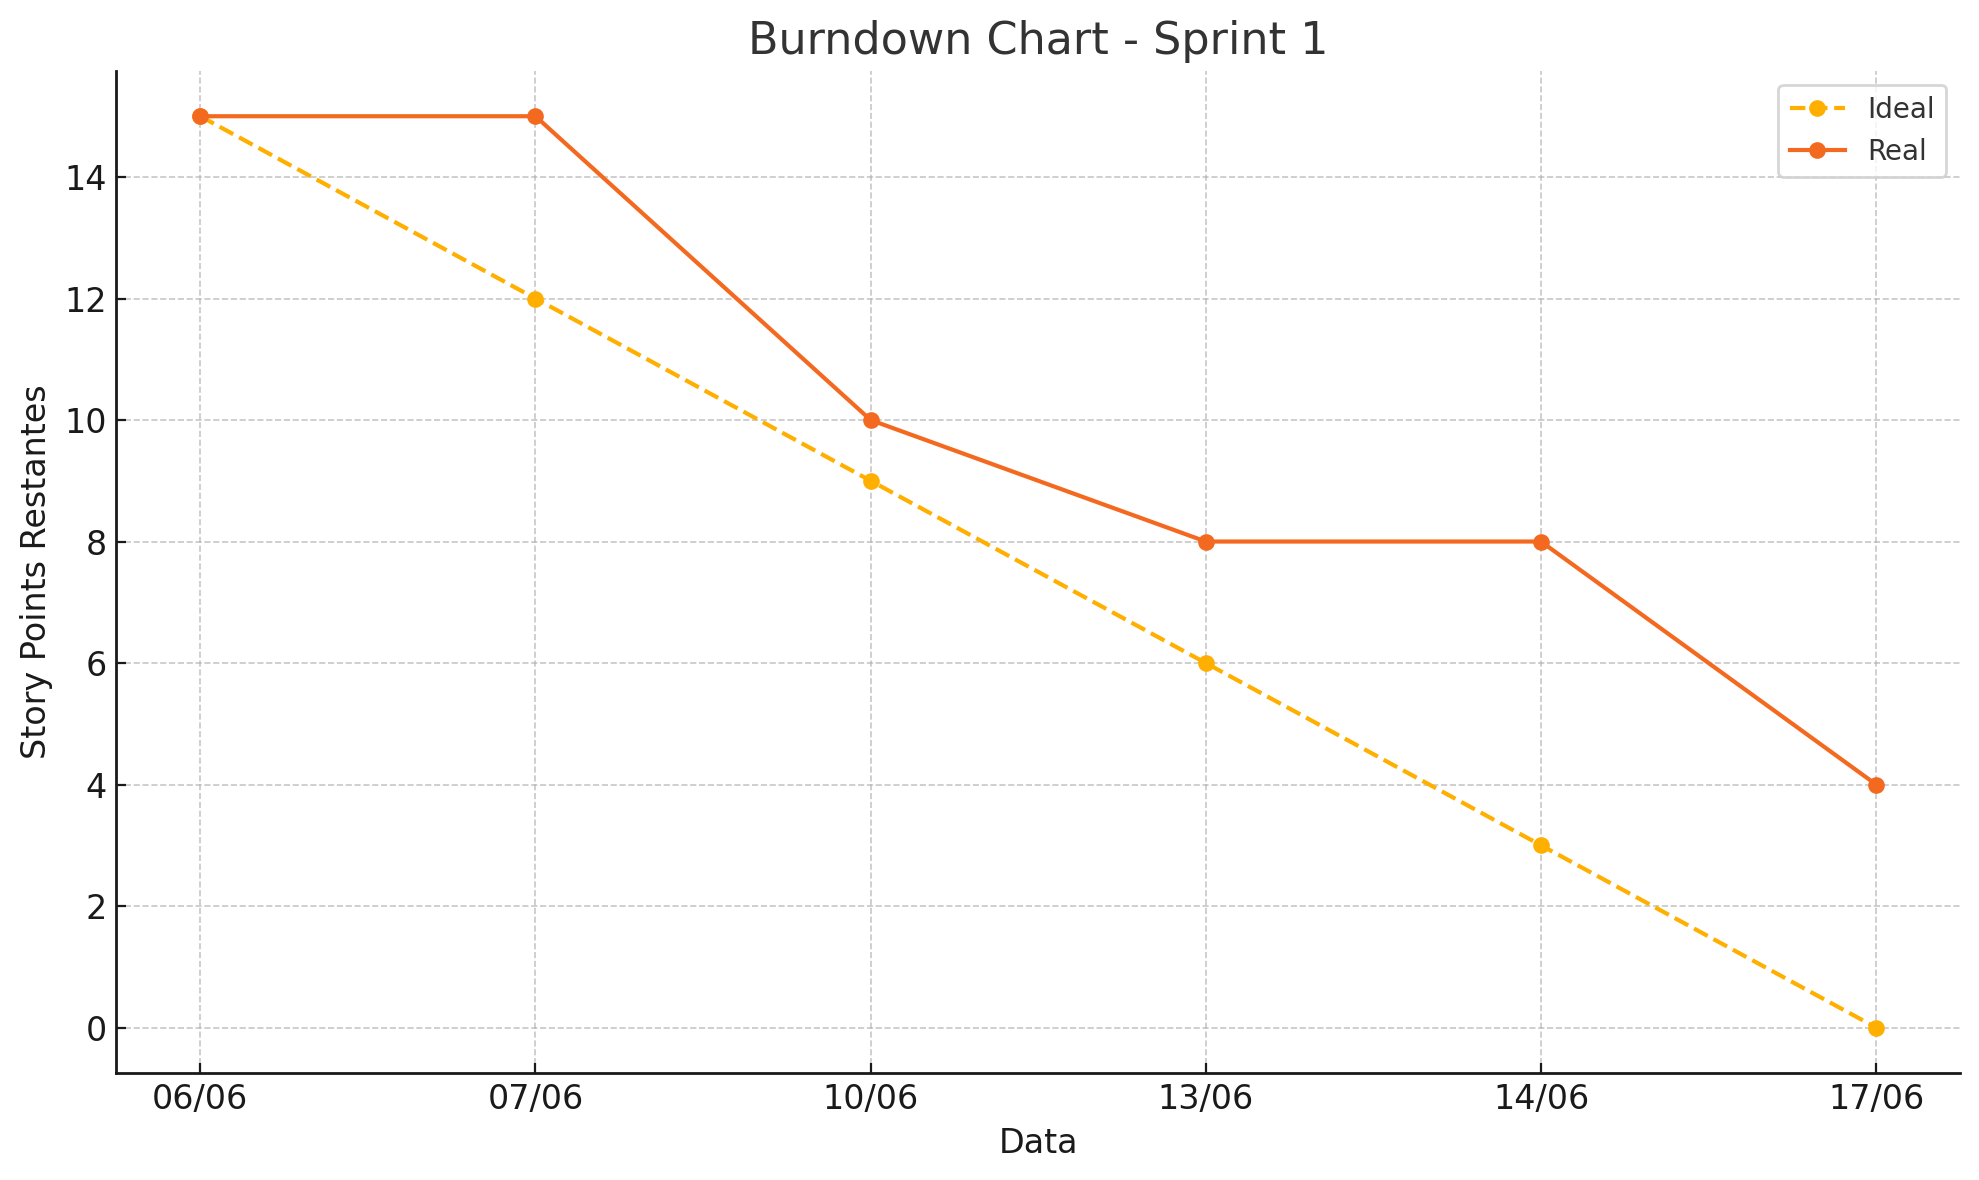
\includegraphics[width=0.7\linewidth]{pictures/burndown_sprint1.png}
  \caption{Burndown — Sprint 1}
\end{figure}


\subsection{Resultados das Sprints}

Essa teve como objetivo principal estruturar a base de fontes bibliográficas para o projeto. Todas as tarefas previstas foram concluídas, embora tenha havido desafios iniciais na definição de critérios de seleção. A equipe conseguiu identificar as três fontes principais a partir de um processo colaborativo de leitura e discussão.

\begin{table}[htbp]
  \centering
  \caption{Resultados — Sprint 1}
  \label{tab:resultSprint1}
  \begin{tabular}{lll}
    \toprule
    ID & Tarefas & Resultado \\
    \midrule
    US-01A & Buscar fontes & Concluída \\
    US-01B & Filtrar fontes & Concluída \\
    US-01C & Selecionar 3 principais fontes & Concluída em 17/06/2025 \\
    \bottomrule
  \end{tabular}
  \fonte{Elaboração própria.}
\end{table}

\vspace{1em}
\noindent\textbf{Resumo da Sprint:}
\begin{itemize}[noitemsep]
  \item Total de tarefas: 3
  \item Concluídas: 3
\end{itemize}

\subsection{Retrospectivas}

\begin{itemize}
  \item \textbf{Pontos de atenção}:
  \begin{itemize}
    \item Baixa adesão às reuniões intermediárias dificultou o alinhamento.
    \item Houve confusão inicial sobre critérios para selecionar artigos relevantes.
  \end{itemize}

  \item \textbf{O que pode ser melhorado}:
  \begin{itemize}
    \item Criar lembretes automáticos das reuniões.
    \item Alinhar expectativas sobre participação mínima esperada de cada integrante.
  \end{itemize}

  \item \textbf{O que manter/continuar}:
  \begin{itemize}
    \item Organização via checklist e Kanban funcionou bem.
    \item Leitura coletiva de fontes-chave ajudou a focar na qualidade da bibliografia.
  \end{itemize}
\end{itemize}

\vspace{1em}
\noindent\textbf{Burndown Chart:}

\begin{center}
  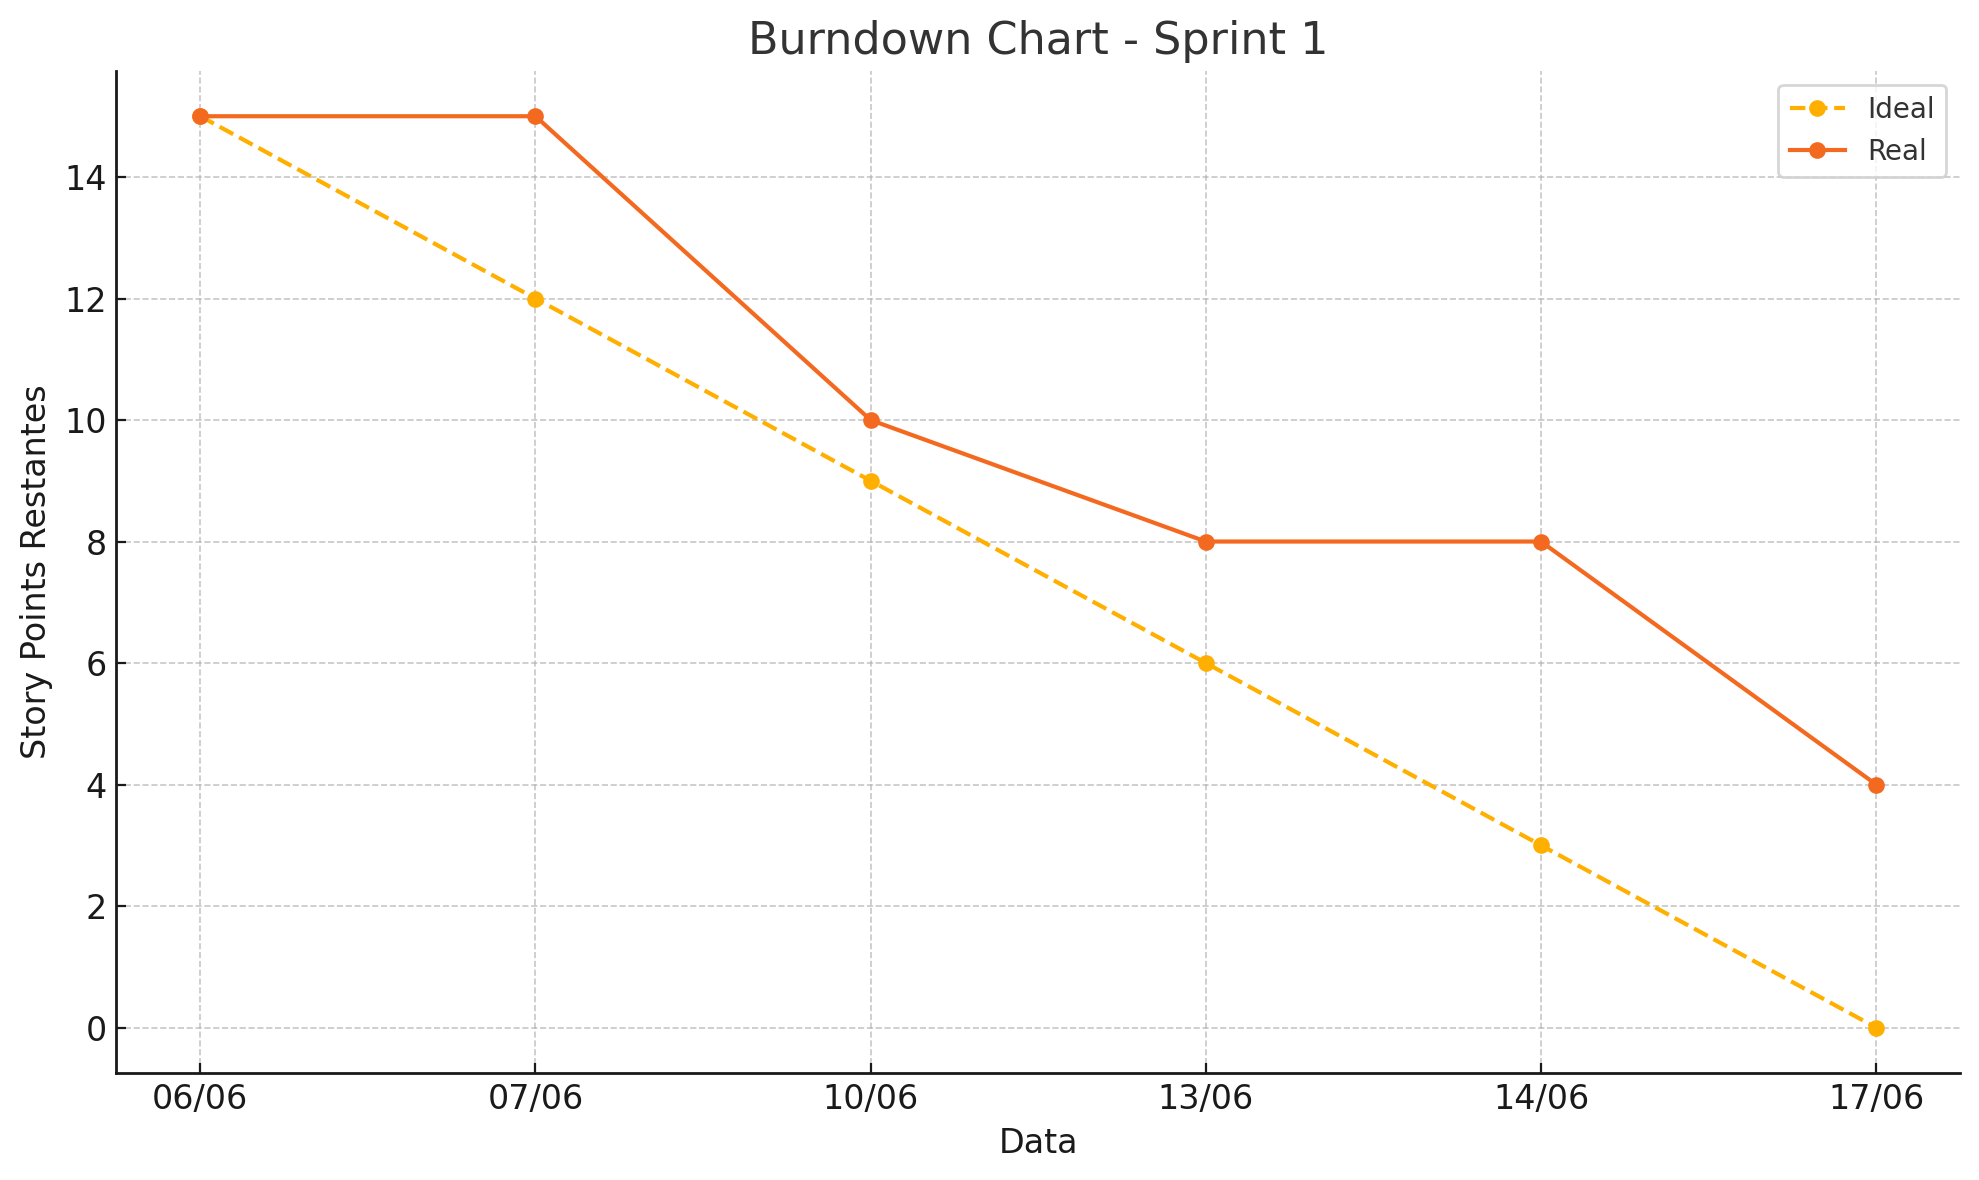
\includegraphics[width=0.8\textwidth]{pictures/burndown_sprint1.png}
\end{center}